\title{VIMS Saturn Occultations: Imaging-Mode Systematics Corrections}
\author{
        Andrew SD Foster
}
\date{}

\documentclass[12pt]{article}

\usepackage{graphicx}

\begin{document}
\maketitle

\begin{abstract}
Cassini performed over 100 occultation experiments in the Saturn system. Most
of these were performed in occultation-mode (using a single pixel to maximize
the temporal resolution of the data). Nine, however, were performed in an
unusual mode (hereafter called "imaging mode") which trades temporal resolution
for additional spatial field-of-view in an effort to better constrain the
refraction physics taking place during these experiments. The wider field-of-
view allows us to observe the star as its image is refracted across the
detector by Saturn's atmosphere. These data allow us to test our assumption
that extinction at wavelengths free of hydrocarbon emission lines is dominated
by differential refraction effects, and potentially to probe for aerosols in
the deep stratosphere. This "imaging mode" used frame-sizes of 16x4 or 16x6
high-resolution pixels, or 8x8 low-resoultion pixels - significantly smaller
than the 64x128 high-resolution pixel or 64x64 low-resolution pixel frames
typically captured by the VIMS instrument ("traditional mode" hereafter). This
unusual mode appears to posses its own systematics, which are difficult to
distinguish from background light sources in the Saturn system. This document
attempts to disentange and correct out these background sources so that these
imaging-mode data may be used.
\end{abstract}

\section{How the VIMS Takes Data}

This section describes how the VIMS instrument takes the image-mode data, and
attempts to highlight parts of the process that likely cause the different
types of errors described below.

\subsection{The Detector}

The VIMS IR detector consists of 256 spectral channels

Talk about the detector, the filter gaps, etc.

\subsection{The Mirror}

Talk about mirror scan times, and how an image is made by raster-scanning the
mirror

\section{Classes of Error}

The errors in these data are a function of some combination of 
There are three classes of errors in these data: Spectral, Spatial,
and Temporal. Of these, Spectral systematics are the easiest to explain and
correct, so we will begin our discussion there.

\subsection{Spectral Systematics}

As described above, one source of systematic error 

\section{Correction Methods for Systematic Errors}

\subsection{Temporal Systematics Corrections}

\subsection{Spatial Systematics Corrections}

\subsection{Hybrid Systematics Corrections}

% Pixel Grid Figure
% \begin{figure}[h!]
% \centering
% 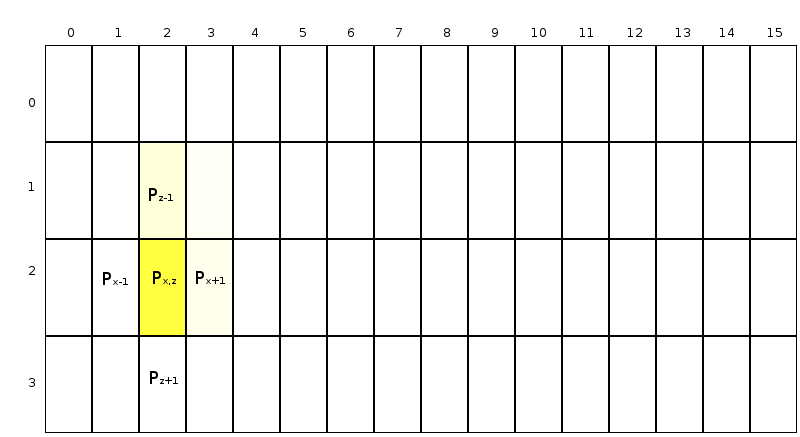
\includegraphics[scale=0.5]{figs/PixelGrid.png}
% \caption{
% The pixels on the Cassini VIMS instrument are 0.5x0.25 $\mathrm{\mu}$radians
% for images taken in the high-resolution mode. They are 0.5x0.5
% $\mathrm{\mu}$radians for images taken in the low-resolution mode. This is a
% diagram of the instrument field-of-view for a 16x4 high-resolution imaging-mode
% occultation, such as that for the AlpOri occultation of rev270s99. The pixels
% used in the calculation of the metric $R$ are labeled. 
% }
% \label{fig:pixels}
% \end{figure}

\end{document}
This is never printed
